\subsection{Tier0}
•Timeline  -- Tier-1 – April 2018

•ipv6      -- readeenes of Tier-1s splitted into LHCOPN, LHCONE, GPI, Monitoring PerfSONAR

•FTS       --- Server status (one out of three only dual-stack)

•Production ipv6 traffic of tier-1 sites
- Triumf is now dual-stackGGUS-ticket-\#:128187 (long standing ticket closed)

• Tier-1 site issues
--  •Transfer issues FTS/gridftp
--  •Dual-homed / Dual-stack  include info of Andreas Petzold + Francesco

In the beginning of 2018, EOS at CERN was upgraded to a version that supported IPv6. 
As soon as the EOS instances of the LHCb and ALICE experiments got a AAAA DNS records for their public nodes, an important increase of IPv6 traffic was noticed on the CERN central firewall, moving from few hundreds of Mbps to almost 10Gbps.

This traffic increase posed some worries, because the IPv6 firewall path was limited to 10Gbps and was actually saturating now and then. So in June 2018 it was implemented the HTAR (High Throughput Alternative Route) firewall bypass also for IPv6, action that has allowed the activation of dual stack access also for the ATLAS and CMS EOS instances. 

The HTAR firewall bypass is a framework that allow some well known, high volume traffic to bypass the statefull inspection of the CERN central firewall. This framework has been in place for many years for IPv4, but the IPv6 part was not implemented initially because of limitation on the network hardware and lately because of a lack of Ipv6 traffic.

Figure \ref{tier0-ipv6-firewall-traffic.png} show the traffic increase when the EOS dual-stack version was introduced

\begin{figure}[h!]
\centering
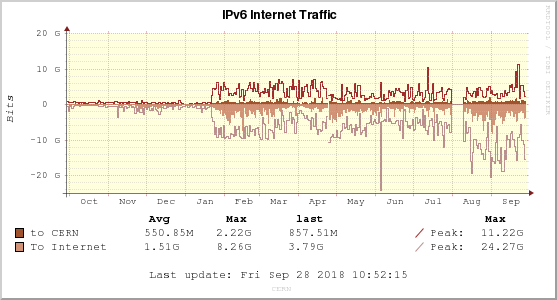
\includegraphics[width=5.6 in]{tier0-ipv6-firewall-traffic.png}
\caption{IPv6 traffic through the CERN central firewall, period Sept 2018-Sept 2019}
\label{fig:tier0-traffic}
\end{figure}
